\subsection{الگوریتم \lr{DDPG}}

الگوریتم \lr{DDPG}  از جمله روش‌های یادگیری خارج از سیاست است که از دو شبکه عصبی برای بازیگر و منتقد استفاده می‌کند. در اینجا، عملکرد نسخه استاندارد و نسخه مبتنی بر بازی مجموع‌صفر این الگوریتم در کنترل فضاپیما مقایسه شده است.

\begin{figure}[H]
	\centering
	
	% سطر اول
	\subfloat[\lr{DDPG} استاندارد]{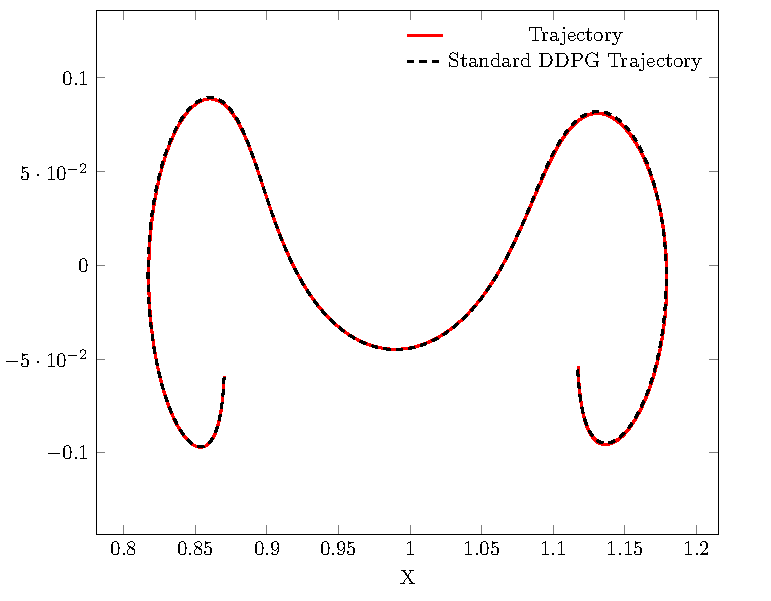
\includegraphics[width=.45\textwidth]{plots/ddpg/trajectory_force/plot_trajectory.pdf}}%
	\subfloat[\lr{DDPG} بازی مجموع‌صفر]{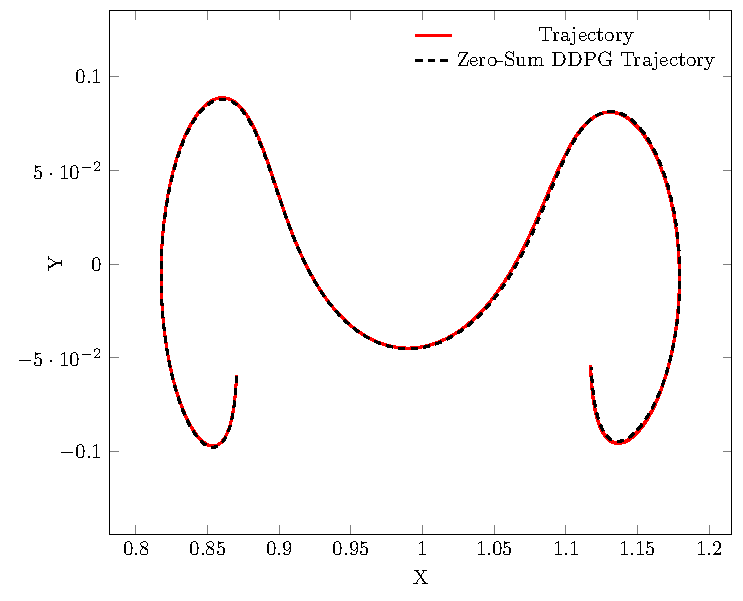
\includegraphics[width=.45\textwidth]{plots/ddpg/trajectory_force/plot_trajectory_zs.pdf}}%
	
	\caption{
		مقایسه مسیر طی شده در دو الگوریتم تک‌عاملی و چندعاملی \lr{DDPG}.
		مشاهده می‌شود که نسخه بازی مجموع‌صفر مسیر مستقیم‌تری را با انحراف کمتر از مسیر بهینه طی می‌کند.
	}
\end{figure}


\begin{figure}[H]
	\centering
	
	% سطر اول
	\subfloat[\lr{DDPG} استاندارد]{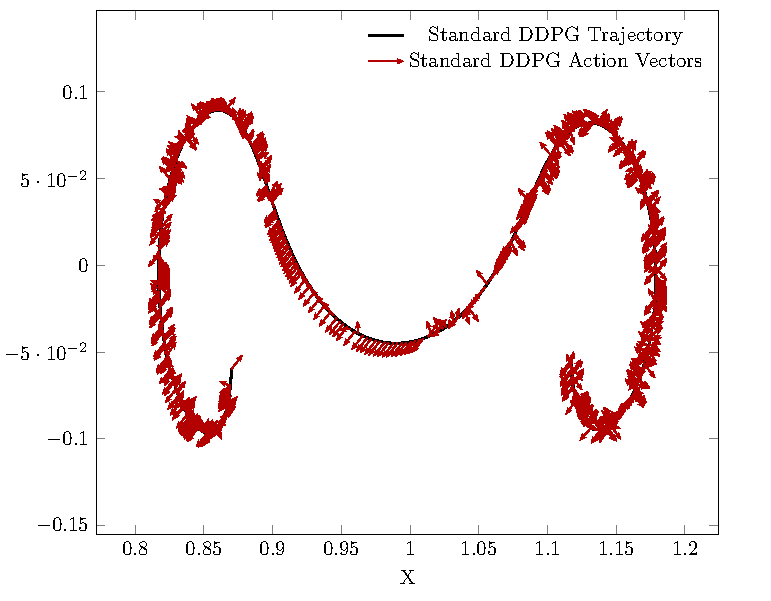
\includegraphics[width=.45\textwidth]{plots/ddpg/trajectory_force/plot_trajectory_force.pdf}}%
	\subfloat[\lr{DDPG} بازی مجموع‌صفر]{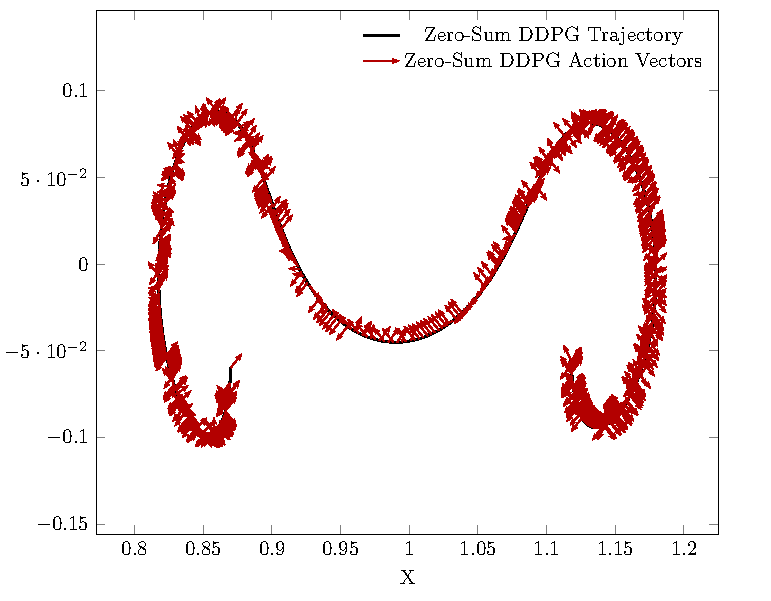
\includegraphics[width=.45\textwidth]{plots/ddpg/trajectory_force/plot_trajectory_force_zs.pdf}}%
	
	\caption{
		مقایسه مسیر و فرمان پیشران دو الگوریتم تک‌عاملی و چندعاملی \lr{DDPG}.
		نمودارهای پایین نشان‌دهنده فرمان پیشران در طول زمان است که در نسخه بازی مجموع‌صفر، الگوی منظم‌تری را نشان می‌دهد و اوج‌های پیشران کمتری دارد.
	}
\end{figure}

همانطور که در شکل‌ها مشاهده می‌شود، الگوریتم \lr{DDPG} مبتنی بر بازی مجموع‌صفر مسیر مستقیم‌تری را طی می‌کند و از نظر مصرف سوخت نیز بهینه‌تر عمل می‌کند. این بهبود عملکرد را می‌توان به ماهیت رقابتی بازی مجموع‌صفر و قابلیت آن در مقابله با عدم قطعیت‌های محیطی نسبت داد.



\subsection{مقایسه الگوریتم‌های تک‌عاملی و چندعاملی \lr{DDPG}}

\begin{figure}[H]
	\centering
	
	% سطر اول
	\subfloat[شرایط اولیه تصادفی]{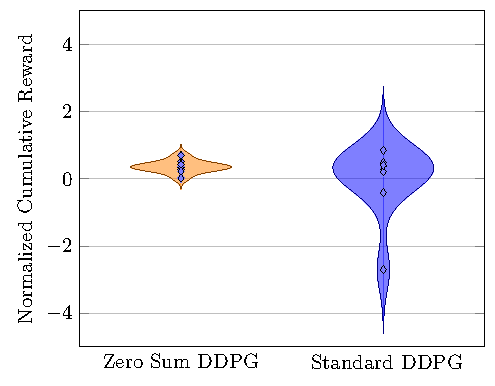
\includegraphics[width=.33\textwidth]{plots/ddpg/violin_plot/initial_condition_shift.pdf}}%
	\subfloat[اغتشاش در عملگرها]{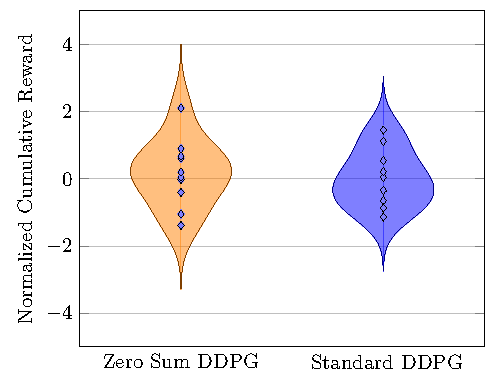
\includegraphics[width=.33\textwidth]{plots/ddpg/violin_plot/actuator_disturbance.pdf}}%
	\subfloat[عدم تطابق مدل]{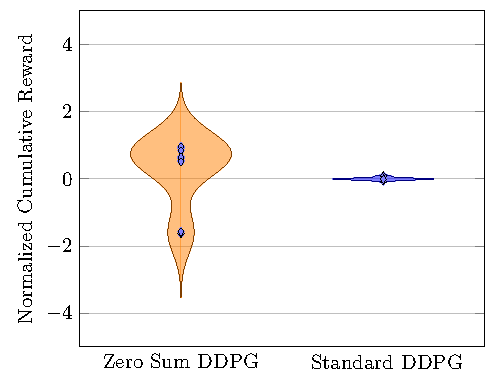
\includegraphics[width=.33\textwidth]{plots/ddpg/violin_plot/model_mismatch.pdf}}\\[1ex]
	
	% سطر دوم
	\subfloat[مشاهده ناقص]{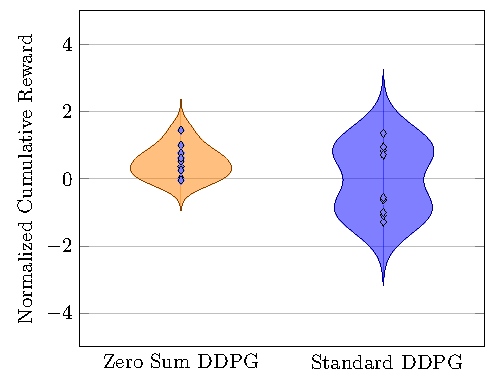
\includegraphics[width=.33\textwidth]{plots/ddpg/violin_plot/partial_observation.pdf}}%
	\subfloat[نویز حسگر]{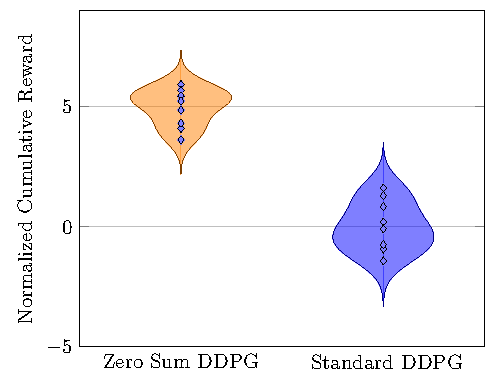
\includegraphics[width=.33\textwidth]{plots/ddpg/violin_plot/sensor_noise.pdf}}%
	\subfloat[تأخیر زمانی]{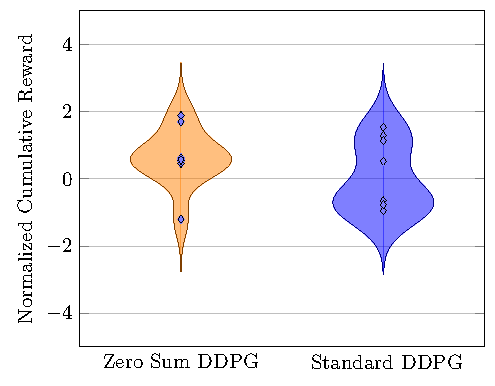
\includegraphics[width=.33\textwidth]{plots/ddpg/violin_plot/time_delay.pdf}}
	
	\caption{مقایسه مجموع پاداش دو الگوریتم تک‌عاملی و چندعاملی \lr{DDPG} در سناریوهای مختلف. 
		نسخه بازی مجموع‌صفر در اکثر سناریوها، به خصوص در شرایط اغتشاش در عملگرها و عدم تطابق مدل، عملکرد بهتری را نشان می‌دهد.
	}
	\label{fig:ddpg_robustness_violin}
\end{figure}

نتایج نشان می‌دهد که الگوریتم \lr{DDPG} مبتنی بر بازی مجموع‌صفر در اکثر سناریوهای چالش‌برانگیز، عملکرد بهتری نسبت به نسخه استاندارد دارد. این برتری به خصوص در شرایط نویز حسگر و شرایط اولیه تصادفی مدل قابل توجه است، که نشان می‌دهد رویکرد چندعاملی توانایی بیشتری در مقابله با عدم قطعیت‌های سیستم دارد.


\begin{table}[H]
	\centering
	\setlength{\tabcolsep}{3pt}
	\small
	\begin{tabular}{@{} R{3.2cm} *{8}{C{1.05cm}} @{}}
		\toprule
		\multirow{2}{*}{\makecell[r]{سناریو}}
		& \multicolumn{2}{c}{پاداش تجمعی} & \multicolumn{2}{c}{مجموع خطای مسیر}
		& \multicolumn{2}{c}{مجموع تلاش کنترلی} & \multicolumn{2}{c}{احتمال شکست} \\
		\cmidrule(lr){2-3}\cmidrule(lr){4-5}\cmidrule(lr){6-7}\cmidrule(lr){8-9}
		& {\rotatebox[origin=c]{90}{\lr{DDPG}}} & {\rotatebox[origin=c]{90}{\lr{MA-DDPG}}}
		& {\rotatebox[origin=c]{90}{\lr{DDPG}}} & {\rotatebox[origin=c]{90}{\lr{MA-DDPG}}}
		& {\rotatebox[origin=c]{90}{\lr{DDPG}}} & {\rotatebox[origin=c]{90}{\lr{MA-DDPG}}}
		& {\rotatebox[origin=c]{90}{\lr{DDPG}}} & {\rotatebox[origin=c]{90}{\lr{MA-DDPG}}} \\
		\midrule
		شرایط اولیه تصادفی
		&
		$-4.17$ & $-3.63$ & $0.40$ & $0.63$ & $5.60$ & $5.60$ & $1.00$ & $1.00$ \\
		اغتشاش در عملگرها
		& $-1.93$ & $-1.96$  & $7.56$ & $7.94$ & $5.60$ & $5.59$ & $0.90$ & $0.30$ \\
		عدم تطابق مدل
		& $-3.24$ & $-2.70$ & $0.70$ & $0.76$ & $5.57$ & $5.57$ & $1.00$ & $1.00$ \\
		مشاهده ناقص
		&
		$-3.28$ & $-2.89$ & $0.68$ & $0.75$ & $5.57$ & $5.57$ & $0.60$ & $0.80$ \\
		نویز حسگر  
		&$-1.07$ & $-0.47$ & $0.10$ & $0.15$ & $5.54$ & $5.54$ & $0.00$ & $0.00$ \\
		تأخیر زمانی        
		&
		$-3.20$ & $-1.91$ & $1.74$ & $2.43$ & $5.61$ & $5.61$ & $0.70$ & $0.70$ \\
		\bottomrule
	\end{tabular}
	\caption{مقایسه عملکرد \lr{DDPG} و \lr{MA-DDPG} در سناریوهای مختلف مقاومت}
	\label{tab:ddpg_comparison}
\end{table}